\chapter{Performance models}

\section{Roofline model}

\todop{Arithmetic vs computational intensity: make this consistent}
%\todop{Weird citation?}

The Roofline model was introduced by \cite{williams-2009}. It is a graph showing two bottlenecks limiting  performance as two lines. The performance is limited either by core execution (horizontal line) or by data transfer (skewed line). Both limits depend on the machine hardware, instructions set used and number of cores.
The name "Roofline model" is inspired by the shape of the graph, as can be seen in Figure \ref{fig:roofline_emmy}:


%The Roofline model~\cite{williams-2009} is a performance model that takes code balance (or arithmetic intensity), attainable performance, and memory bandwidth as input and predicts the performance of the code on a given machine. It assumes the performance is limited either by core execution or by data transfer. The name "Roofline model" is inspired by the shape of the graph, as can be seen in Figure \ref{fig:roofline_emmy}:

\begin{equation}
   P = min(P_{max}, I \cdot b_s) = min(P_{max}, b_s / B_c),
\end{equation}

\noindent
where $P [F/s]$ is the expected performance.
Attainable performance $P_{max} [F/s]$ depends on the CPU and on the code. In the best case, it is equal to peak performance, but it can also be lower, for example, if the code does not use vector instructions. $I [F/B]$ is computational intensity (code balance $B_c = I^{-1}$). And the memory bandwidth $b_s [B/s]$ can be found in the datasheet or measured with the microbenchmark.

\begin{figure}[H]
   \centering
   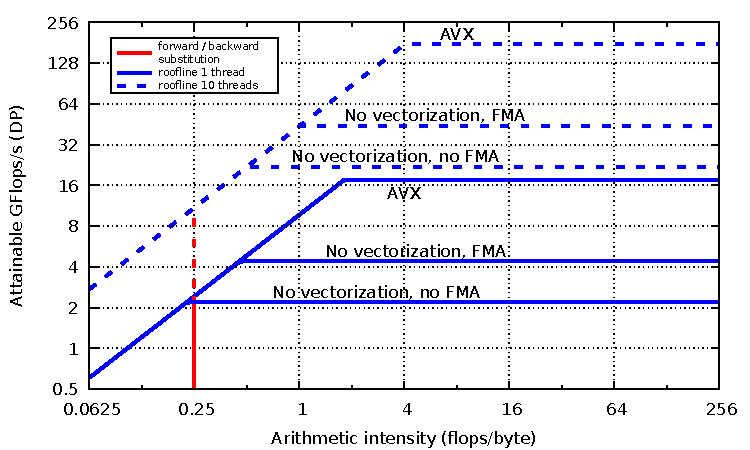
\includegraphics[width=0.7\textwidth,clip=true]{images/roofline_emmy_Xeon2660v2}
   \caption{Roofline model of the  Intel Xeon E5-2660 v2 CPU. \todol{replace with tikz}}
  \label{fig:roofline_emmy}
\end{figure}

The limits are given only by the machine characteristics, it can be created once for one machine. For given algorithm, knowing its operational intensity, we can easily find out its maximum performance that can be achieved and which of the two factors limit the performance.

\section{Extended roofline model}
\label{sec:mrm}

% \begin{table}[tp]
%   \centering
%   \small
%   \begin{tabular}{l|cccc}
%   \hline
%   u & l1 & l2 & l3 & mem \\
%   \hline
%   forward \\
%   \hline
%   1 & 14   & 4 -- 14  &  4 -- 14  & 4 -- 6    & \\
%   2 &  9   & 4 --  9  &  4 --  9  & 4 -- 5    & \\
%   8 & 5.25 & 4 -- 5.25&  4 -- 5.25& 4 -- 4.25 & \\
%   \hline
%   backward \\
%   \hline
%   1 & 10  & 4 -- 10 & 4 -- 10 & 4 -- 6 \\
%   2 & 7   & 4 --  7 & 4 --  7 & 4 -- 5 \\
%   8 & 4.75& 4 -- 4.75&4--4.75& 4 -- 4.25\\
%   \end{tabular}
%   \caption{code balance $b_c$ [b/flop] of forward/backward substitution for
% different unrollings (u) when
% data is fetched from the corresponding level inside the memory hierarchy. values
% depend on actual panel size $s$ and possible cache reuse.}
%   \label{tab:mrm:bc}
% \end{table}

The roofline model is very useful for code that is either completely sequential or completely parallel. However when code cannot be completely parallelized, the roofline model cannot be used, because the attainable performance $P_{max}$ and memory bandwidth $b_s$ depend on number of threads used.
%The model takes into account the attainable memory bandwidth and peak floating
%point performance of the processor and correlates it with the requirements of
%the code.
%It can be written as
%%
%\be
%  P = \min(P_\text{max}, B / B_c),
%\ee
%where $P_\text{max}$ denotes the attainable floating point performance, $B$ the
%attainable memory bandwidth and $B_c$ the \textit{code balance}.
%Here $P_\text{max}$
%depends already on the floating point characteristics of the code. 
%First it depends on the usage of vector or scalar instructions in the code.

One should also take into account the instruction set.
In our case only scalar instructions are used, which for example quarter the
theoretically attainable floating point performance for a processor supporting
AVX.
Furthermore if floating point units for addition and multiplication are
separated and the code uses only one type of these operation the attainable
performance is furthermore halfed.

We modified the roofline model such that it models independently the work done sequentially and in parallel.
The formula used for combination of $1$ and $t$ threads is
%
\begin{equation}
  p^{a}(t) 
  = \frac{
      f
    }{
     \frac{d_a^p(t) }{  b(t) } + \frac{ d_a^s(t) }{ b(1) }
    } \left[ \frac{\text{flop}}{s} \right],
\end{equation}
%
where $f$ denotes the total number of floating point operations,
$b(t)$ is the attainable memory bandwidth with $t$ threads,
$b(1)$ is the attainable memory bandwidth with $1$ thread,
$d_a^p(t)$ the data volume of nonzeros and indices made up by the parallel 
parts, and $d_a^s(t)$ the data volume made up by the nonzeros and indices of the
sequential computation (separator).



\section{ECM model}

\noindent
\todop{
\begin{itemize}
    \item Memory bandwidth limited codes
    \item Stencil codes
    \item Assumption from where the data come from
    \item Limits from different levels of the memory hierarchy (M, L3, L2, L1)
\end{itemize}
}

The Execution Cache Memory model (ECM) predicts number of CPU cycles required to execute a certain number of iterations of a given loop on a single core. As the smallest amount of data copied between cache levels is one cache line (CL), it is reasonable unit of work for the predictions. The size of cache line on Intel processors is 64\,B, which is for streaming kernels 8 iterations with real numbers in double precision.

To construct the model, we consider two parts separately: the in-core execution, assuming all data were already fetched to L1 cache and there are no cache misses, and the time to fetch the data from the main memory or the cache level where it is assumed to be stored to L1 cache.

To determine the in-core execution time, some knowledge about the architecture is required. Detailed description of Intel architectures can be found in the Intel Optimization Reference Manual \todol{add citation https://www.intel.com/content/dam/www/public/us/en/documents/manuals/64-ia-32-architectures-optimization-manual.pdf}. Simple kernels without loop-carried dependencies can be modelled manually. We assume all instructions in the loop are scheduled to the ports and executed out of program order. \todol{max 4 instructions (micro-ops) per cycle}
When the kernel is more complicated, obtaining precise results manually becomes unfeasible, as the scheduling and data dependency between instructions can be very complicated. In such cases Intel Architecture Code Analyser (IACA) \todol{add reference https://software.intel.com/en-us/articles/intel-architecture-code-analyzer} can be used to analyze the code.

Before the data can be loaded in the CPU register, it must be fetched to L1 cache and after the processing it must be evicted back to the original location to make space for another data. This is called  the "transfer time".

The predictions are done for single core. When multiple cores are used, the core execution scales perfectly. Bottleneck can be reached on data transfers from cache that is shared between threads or main memory.

\subsection{Aplication of ECM on a simple example}

Let's illustrate the ECM model on a simple DAXPY kernel on Intel Sandy Bridge architecture, taken from \todol{cite the ECM paper}.
\begin{lstlisting}[language=C]
for(i=0; i<N; ++i)
    a[i] = a[i] + s*b[i];
\end{lstlisting}
\todop{add Sandy Bridge ports image}

Execution of 8 iterations of this loop with AVX vectorization needs four load, two store, two multiply and two add instructions. This requires four cycles. There are also integer add and compare for the loop mechanics, which can be neglected.

On the Intel Sandy Bridge architecture transferring one cache line between adjacent cache levels takes two cycles.
Transferring a cache line from memory to L3 cache or back takes $64\,B \cdot f/ BW$, where $f$ is the CPU frequency and $BW$ is a bandwidth measured by a benchmark. With frequency 2.7\,GHz and bandwidth 40\,GB/s, we get 4.3 cy/CL.

For the DAXPY kernel we need to transfer 3 CL (loading a and b, evicting a). Transfering this data between L1-L2 and L2-L3 takes 6 cycles, L3-mem takes 13 cycles. These transfers cannot overlap.

With the data above we can construct the ECM model of the DAXPY kernel for single thread.

\begin{eqnarray}
    T_{core} & = & \max(T_{nOL}, T_{OL}) \\
    T_{ECM} & = & \max(T_{nOL}+T_{data}, T_{OL}) \label{eq:ecm}
\end{eqnarray}
Where $T_{data}$ is the transfer time from location where the data are stored to L1 cache, $T_{nOL}$ is the part of the core execution that does not overlap with the transfer time and $T_{OL}$ is the part that overlaps with the transfer time.

\todop{par otazek viz paper}
\todop{ECM notation}
The information from the figure \todol{ref ECM figure} can be represented by the following notation:
\begin{equation}
    \{T_{OL} || T_{nOL} | T_{L1L2} | T_{L2L3} | T_{L3Mem}\}
\end{equation}

For the DAXPY example it is $\{\,4\,||\,4\,|\,6\,|\,6\,|\,13\,\}\,cy$.
From this representation $T_{data}$ can be calculated for any location where the data reside by adding all the appropriate tranfer times.
Then the ECM prediction by equation \ref{eq:ecm} is $T_{ECM} = \{4 \rceil 10 \rceil 16 \rceil 29\} cy$, where $\rceil$~delimiters prediction for data coming from L1, L2, L3 cache and memory respectively.

\todop{add and ref Figure 2 from the ECM paper}